\documentclass{beamer}

\usepackage[english]{babel}

\usepackage[latin1]{inputenc}

\usepackage{times}
\usepackage{hyperref}
\usepackage{listings}
\usepackage{comment}
\usepackage{booktabs} % for toprule
\usepackage{tikz}
\usetikzlibrary{positioning}

\lstset{frame=none, showstringspaces=false, basicstyle=\footnotesize,
  xleftmargin=-6mm,language=Haskell}

\newcommand{\colAwidth}{0.1\textwidth}
\newcommand{\colBwidth}{0.8\textwidth}

\title[GOOL]{Multi-lingual code generation in Drasil}

\author{\underline{Jacques Carette}, Spencer Smith, Dan Szymczak and
Steven Palmer}

\institute[McMaster University]{McMaster University}

\date[July 2017]{WG 2.11, July 2017 Meeting}

\beamertemplatenavigationsymbolsempty 

\begin{document}

%I will present some ongoing work that seeks to generate all the artifacts
%involved in software (obviously code, but also specification documents, design
%documents, tests, user manual, Makefiles, etc). In the context of software
%which requires (re)certification, all of these artifacts are involved -- and
%they normally contain a huge amount of duplicate information. Our approach is
%to do very aggressive knowledge encapsulation, followed by relatively
%straightforward generation passes. For domains (such as scientific computation)
%where there is well-established theory, our preliminary experiments shows that
%this works quite well. Note that we do NOT expect this to work so well in
%domains without well-established theory.

\begin{frame}
\titlepage
\end{frame}

\begin{frame}

\includegraphics{generate_all_the_things.jpg}
\end{frame}

\begin{frame}

\includegraphics[width=\textwidth]{no_silver_bullet.jpg}
\end{frame}

% Drasil
%%% - generate all the things
%%% - no silver bullet
%%% - context
%%% * example: doc (D) + code (S) (GlassBR)
%%% - ontologies (D)
%%%   * go through well-formatted Data.Drasil.Concepts.*, Data.Drasil.SI_Units
%%%       (D - if you could make sure these are as clean as possible?)
%%%   - typeclasses of Language.Drasil (D) [esp. as this has evolved a lot recently]
%%%   * Example.Drasil.DocumentLanguage.

\begin{frame}
\frametitle{Context}
{\Large software \onslide<2->{(re)}certification}
\vspace*{.2cm}
\begin{itemize}
\item<3->All software artifacts as \textcolor{green}{evidence}:
\begin{itemize}
\item \textcolor{blue}{requirements, software specification, software design, code, 
  tests, ``theory manual'', user manual, \ldots}
\end{itemize}
\vspace*{.5cm}
\item<4->Massive amounts of \textcolor{red}{knowledge duplication}
\begin{itemize}
  \item Implies that either
  \begin{itemize}
    \item non-code artifacts do not get maintained well enough, OR
    \item are felt to be an expensive nuisance
  \end{itemize}
  \item duplication harms traceability
\end{itemize}
\end{itemize}
\vfill
\end{frame}

\begin{frame}
\frametitle{Examples}
\begin{itemize}
\item {\color{blue}GlassBR}: Computer whether a given plate of glass will resist a blast force.
\item GamePhysics: ``Chipmunk'' game physics engine.
\item SSP: Computation of mixed-soil slop stability.
\item SWHS: Solar Water Heating System (w/ phase change material).
\item NoPCM: Solar Water Heating System without PCM.
\item Tiny: convective and effective heat transfer coefficients.
\end{itemize}
\end{frame}

\begin{frame}[t]
\frametitle{Ontologies}
{\large \onslide<1->{\only<1>{\color{blue}}Data.Drasil} 
\onslide<2,3->{- \only<2>{\color{blue}}Language Concepts}
\onslide<3->{- \only<3->{\color{blue}}Document Language}}

\only<1>{
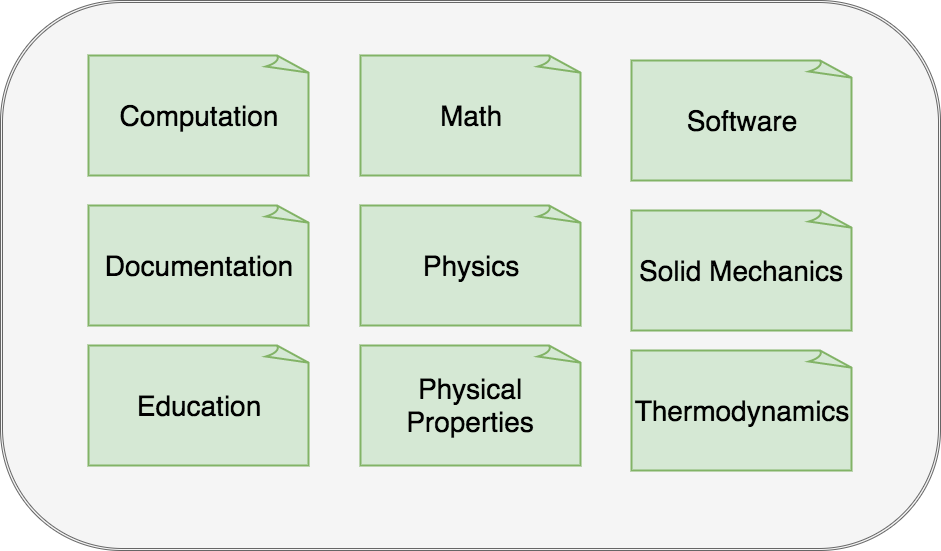
\includegraphics[scale=0.33]{Data_Drasil.png}
}
\only<2>{
\center{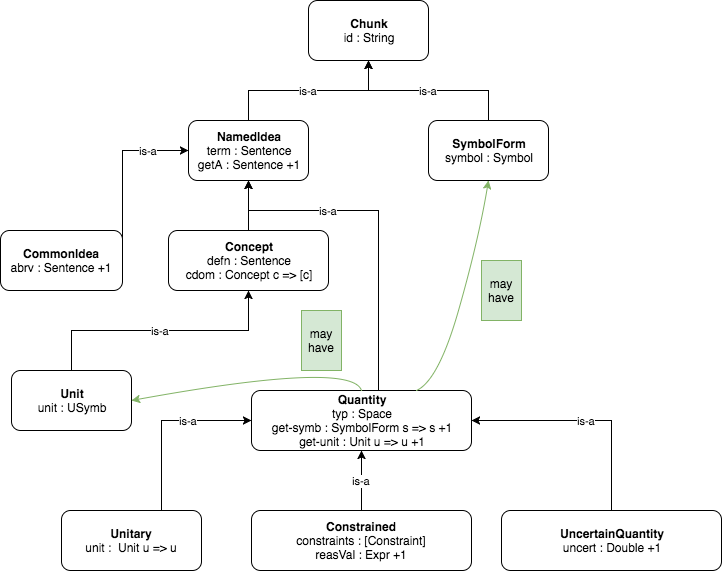
\includegraphics[scale=0.33]{class_hierarchy.png}}
}
\only<3>{
\vspace{2cm}
\emph{\Large{Show the details already!}}
}
\end{frame}

\begin{frame}
\frametitle{GOOL}
{\Large {\color{blue}G}eneric {\color{blue}O}bject-{\color{blue}O}riented {\color{blue}L}anguage.}

History:
\begin{itemize}
\item Lucas Beyak
\item Jason Costabile
\item Yuriy Toporovskyy
\end{itemize}
\pause
Currently covers
\begin{itemize}
\item Java, C\#
\item C++
\item Python, Lua
\item Objective-C
\item GOOL
\end{itemize}
\end{frame}

\begin{frame}[plain, fragile]
\frametitle{GOOL Design}
{\Large Requirements}
\begin{enumerate}
\item Capture the essence of programming in mainstream, pseudo-OO languages.
\item Make the embedded DSL palatable.
\item Eschew language-specific ``idiomatic'' patterns.
\item Target for generation.
\end{enumerate}
\pause
\begin{itemize}
\item multiple languages implies GOOL must capture
\begin{itemize}
\item<3-> features common to all targeted languages\onslide<3->{, and}
\item<4-> \emph{language-required} features not common to all languages:
\begin{itemize}
\item public/private scoping
\item dynamic/static binding
\item explicit destructors
\item explicit types in IO statements
\end{itemize}
\end{itemize}
\item<5-> when rendering, extra information can be dropped
\end{itemize}
\end{frame}

\begin{frame}[plain, fragile]
\frametitle{GOOL Design}
{\Large Renderer}
\begin{itemize} 
\item uses data type that acts as virtual dispatch table:
\begin{lstlisting}
    data Config = Config {
      assignDoc :: Assignment -> Doc,
      binOpDoc :: BinaryOp -> Doc,
      bodyDoc :: Body -> Doc,
      blockDoc :: Block -> Doc,
      callFuncParamList :: [Value] -> Doc,
      conditionalDoc :: Conditional -> Doc,
      declarationDoc :: Declaration -> Doc,
      exprDoc :: Expression -> Doc,
      funcDoc :: Function -> Doc,
      -- and many more
    }
\end{lstlisting}
\item each of the 7 languages has its own Config that uses a different set of rendering functions
\item Text.PrettyPrint package used to make rendered code look nice
\end{itemize}
\end{frame}


\begin{frame}[plain, fragile]
\frametitle{GOOL Design}
{\Large GOOL syntax}
\begin{itemize}
\item designed to look like a programming language by using
\begin{enumerate}
\item<2-> custom infix operators:
\begin{lstlisting}
    -- logical operators
    (?!), (?<), (?<=), (?>), (?>=), -- etc.
    -- arithmetic operators
    (#~), (#/^), (#|), (#+), (#-), -- etc.
    -- assignment operators
    (&=), (&-=), (&++), (&~-) -- etc.
\end{lstlisting}
\item<3-> smart constructors:
\begin{lstlisting}
  bool, int, float, char, string,
  true, false,
  pubClass, privClass, 
  pubMethod, privMethod,
  print, printLn
\end{lstlisting}
and so on (about $100$).
\end{enumerate}
\end{itemize}
\end{frame}

\begin{frame}[plain, fragile]
\frametitle{GOOL Design}
Consider the function $f(x, y) = 2x/y$.  In GOOL:
\begin{lstlisting}
f :: FunctionDecl
f = pubMethod (methodType float) "f"
  [param "x" float, param "y" float] 
  (oneLiner $ return $ 
    (litFloat 2) #* (var "x") #/ (var "y"))
\end{lstlisting}
\end{frame}


\begin{frame}[plain, fragile]
\frametitle{Choices}
{\Large Some implementation choices}
\begin{itemize}
\item programming language to be rendered?
\pause
\item generate library or program?
\pause
\item logging?
\begin{itemize}
\item function calls
\item variable assignments
\end{itemize}
\pause
\item documentation in code?
\begin{itemize}
\item commented classes
\item commented functions
\item commented variables 
\end{itemize}
\end{itemize}
\end{frame}

\begin{frame}[plain, fragile]
\frametitle{Choices}
{\Large Some design choices}
\begin{itemize}
\item structure of input/output?
\begin{itemize}
\item file vs console
\item how data is arranged
\end{itemize}
\pause
\item behaviour on failed constraints?
\begin{itemize}
\item print warning
\item quit with error
\item throw exception
\end{itemize}
\pause
\item which (common) algorithms to use?
\begin{itemize}
\item choice of sorting algorithm
\item choice of searching algorithm
\item etc.
\end{itemize}
\end{itemize}
\end{frame}



% Gool
%%% - origins (J)
% - design
%   - meta-language abstracting details (J)
%     - all required features of all languages (S?)
%        ex: public/private
%     - 7 language renderers (as virtual dispatch table - in Haskell!) (S)
%     - pretty-printer to make things look nice
%     - lots of smart constructors to make it look PL-like (give example) (S)
% 
% Choices
% - implementation choices, design choices, "aspects" (J)
% - examples of
%   - implementation choices (S)
%   - design choices (S) 

\begin{frame}

\includegraphics[width=0.48\textwidth]{generate_all_the_things.jpg}

\includegraphics[width=0.48\textwidth]{no_silver_bullet.jpg}
\end{frame}

\end{document}
